\documentclass[10pt,a4paper]{article}
\usepackage{amsmath}
\usepackage{amssymb}
\usepackage{graphicx}
\usepackage{color}
\usepackage{fancyhdr}
\usepackage{fancyvrb}
\usepackage[margin=3.5cm]{geometry}
\usepackage{framed}
\usepackage{enumerate}
\usepackage{textcomp}
\def\ket#1{\left|#1\right\rangle}
\def\bra#1{\left\langle#1\right|}
\def\braket#1{\left\langle#1\right\rangle}

\FrameSep 8pt
\setlength{\topsep}{1pt}

\definecolor{linkcol}{rgb}{0.0, 0.0, 0.5}
\usepackage[colorlinks=true,urlcolor=linkcol,citecolor=black,linkcolor=linkcol]{hyperref}

\renewcommand\thesection{9.\arabic{section}}
\renewcommand\thesubsection{\thesection.\arabic{subsection}}

\fancyhf{}
\lhead{\tiny Y.~D.~Chong (2016)}
\rhead{\scriptsize MH2801: Complex Methods for the Sciences}
\lfoot{}
\rfoot{\thepage}
\pagestyle{fancy}

\makeatletter
\def\PY@reset{\let\PY@it=\relax \let\PY@bf=\relax%
    \let\PY@ul=\relax \let\PY@tc=\relax%
    \let\PY@bc=\relax \let\PY@ff=\relax}
\def\PY@tok#1{\csname PY@tok@#1\endcsname}
\def\PY@toks#1+{\ifx\relax#1\empty\else%
    \PY@tok{#1}\expandafter\PY@toks\fi}
\def\PY@do#1{\PY@bc{\PY@tc{\PY@ul
\def\PYZdl{\char`\$}
\def\PYZhy{\char`\-}
\def\PYZsq{\char`\'}
\def\PYZdq{\char`\"}
\def\PYZti{\char`\~}

\begin{document}
\setcounter{page}{68}
\noindent
\underline{\textbf{\LARGE 9. Fourier Series and Fourier Transforms}}
\vskip 0.1in
    
The \textbf{Fourier transform} is one of the most important tools for
analyzing functions. The basic underlying idea is that a function
$f(x)$ can be expressed as a linear combination of elementary
functions (specifically, sinusoidal waves). The coefficients in this
linear combination can be regarded as a counterpart function, $F(k)$,
that is defined in a wave-number domain $k \in \mathbb{R}$. This is
helpful because certain mathematical problems, such as differential
equations, are easier to solve in terms of $F(k)$ rather than directly
in terms of $f(x)$.

\section{Fourier series}\label{fourier-series}

We begin by discussing the \textbf{Fourier series}, which is used to
analyze functions which are periodic in their inputs. A \textbf{periodic
function} $f(x)$ is a function of a real variable $x$ that repeats
itself every time $x$ changes by $a$, as in the figure below:

\begin{figure}[h]
  \centering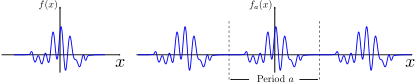
\includegraphics[width=0.6\textwidth]{periodicity}
\end{figure}

The constant $a$ is called the \textbf{period}. Mathematically, we
write this condition as
\begin{equation}
  f(x+a) = f(x), \;\; \forall\; x\in \mathbb{R}.
\end{equation}
In a physical context, the value of $f(x)$ can be either real or
complex. We will assume that the input variable $x$ is real, and that
it refers to a spatial coordinate. (Most of the following discussion
can also apply to functions of time, with minor differences in
convention that \hyperref[fourier_time]{we'll discuss later}.)

We can also think of a periodic function as being defined over a domain
of length $a$, say $-a/2 \le x < a/2$. The periodicity condition is
equivalent to joining the edges of the domain to form a ring of
circumference $a$, as shown in the figure below. Then the position
along the circumference of the ring serves as the $x$ coordinate.

\begin{figure}[h]
  \centering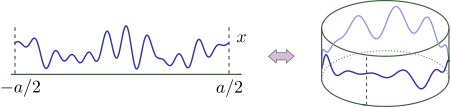
\includegraphics[width=0.6\textwidth]{periodic_function}
\end{figure}

Consider what it means to \emph{specify} an arbitrary periodic
function $f(x)$. One way to specify the function is to state its value
for every $-a/2 \le x < a/2$. But that's an uncountably infinite set
of numbers, which is cumbersome to deal with. A better alternative is
to express the function as a linear combination of simpler periodic
functions, such as sines and cosines:
\begin{equation}
  f(x) = \sum_{n=1}^\infty \alpha_n \sin\left(\frac{2\pi n x}{a}\right) + \sum_{m=0}^\infty \beta_m \cos\left(\frac{2 \pi m x}{a}\right).
\end{equation}
This is called a \textbf{Fourier series}. If $f(x)$ can be expressed
as such a series, then it can be fully specified by the set of numbers
$\{\alpha_n, \beta_m\}$, which are called the \textbf{Fourier
  coefficients}. These coefficients are real if $f(x)$ is a real
function, or complex if $f(x)$ is complex-valued. (Note that the sum
over $n$ starts from 1, but the sum over $m$ starts from 0; that's
because the sine term with $n = 0$ is zero for all $x$, so it's
redundant.) The justification for the Fourier series formula is that
these sine and cosine functions are themselves periodic, with period
$a$:
\begin{align}
  \sin\left(\frac{2\pi n (x+a)}{a}\right) = \sin\left(\frac{2\pi n x}{a} + 2\pi n\right) &= \sin\left(\frac{2\pi n x}{a}\right)
  \\ \cos\left(\frac{2\pi n (x+a)}{a}\right) = \cos\left(\frac{2\pi n x}{a} + 2\pi n\right) &= \cos\left(\frac{2\pi n x}{a}\right)
\end{align}
Hence, any such linear combination satisfies the periodicity condition
$f(x+a) = f(x)$ automatically.

The Fourier series is a nice way to specify periodic functions,
because we only need to supply the Fourier coefficients $\{\alpha_n,
\beta_m\}$, which are a discrete set of numbers; then the value of
$f(x)$ is completely determined for all $x$. Although the set of
Fourier coefficients is formally infinite, in many cases the Fourier
coefficients are negligible for large $m$ and $n$ (corresponding to
very rapidly-oscillating sine and cosine waves), so we only need to
keep track of a small number of low-order coefficients.

\subsection{Square-integrable functions}
\label{square-integrable}

For a function $f(x)$ to be expressible as a Fourier series, the
series needs converge to $f(x)$ as we sum to infinity. Under what
circumstances does convergence occur?
\href{http://en.wikipedia.org/wiki/Convergence_of_Fourier_series}{The
full answer to this question turns out to be long and difficult}, and we
will not go into the details. Luckily, most periodic functions
encountered in physical contexts do have convergent Fourier series. In
fact, they are usually part of a class of functions called
\textbf{square-integrable functions}, which are \emph{guaranteed} to
have convergent Fourier series.

Square-integrable functions are those for which the integral
\begin{equation}
  \int_{-a/2}^{a/2} dx\; \big|\,f(x)\,\big|^2
\end{equation}
exists and is finite. From now on, we will simply assume that we're
dealing with functions of this sort, and not worry about the issue of
convergence.

\subsection{Complex Fourier series and inverse relations}
\label{complex-fourier-series}

Using Euler's formula, we can re-write the Fourier series as follows:
\begin{equation}
  f(x) = \sum_{n=-\infty}^\infty e^{2\pi i n x/a}\, f_n.
\end{equation}
Instead of separate sums over sine and cosine functions, we sum over
complex exponential functions. We have a new set of Fourier
coefficients, $f_n$, and the sum includes negative integers $n$.  This
form of the Fourier series is a lot more convenient to work with,
since we now only have to keep track of a single sum rather than
separate sums for the sine and cosine terms.  (As an exercise, try
working out the explicit relationship between the old and new
coefficients.)

The above Fourier series formula tells us that if the Fourier
coefficients $\{f_n\}$ are known, then $f(x)$ can be determined. The
converse is also true: if we are given $f(x)$, it is possible for us
to determine the Fourier coefficients. To see how this is done, first
observe that
\begin{equation}
  \int_{-a/2}^{a/2} dx \; e^{-2\pi i m x/a}\, e^{2\pi i n x/a}
  = a\, \delta_{mn}\quad \mathrm{for}\;m, n \in \mathbb{Z},
\end{equation}
where $\delta_{mn}$ is the
\href{http://en.wikipedia.org/wiki/Kronecker_delta}{Kronecker delta},
defined as:
\begin{equation}
  \delta_{mn} = \left\{\begin{array}{ll}1, & \textrm{if}\; m = n
  \\ 0, & \mathrm{if}\;m\ne n.\end{array}\right.
\end{equation}
Due to this property, the set of functions $\exp(2\pi i n x / a)$,
with integer values of $n$, are said to be \textbf{orthogonal}
functions. (We won't go into the details now, but the term
``orthogonality'' is used here with the same meaning as in vector
algebra, where a set of vectors $\vec{v}_1, \vec{v}_2, \dots$ is said
to be ``orthogonal'' if $\vec{v}_m \cdot \vec{v}_n = 0$ for $m\ne n$.)
Using this result, we can show that
\begin{align}
  \int_{-a/2}^{\,a/2} dx\; e^{-2\pi i m x/a} \;f(x)
&= \, \int_{-a/2}^{\,a/2} dx\; e^{-2\pi i m x/a} \left[\sum_{n=-\infty}^\infty e^{2\pi i n x/a}\, f_n\right] \\
&= \sum_{n=-\infty}^\infty \, \int_{-a/2}^{\,a/2} dx\; e^{-2\pi i m x/a}  \, e^{2\pi i n x/a} \;f_n \\
&= \sum_{n=-\infty}^\infty \, a\, \delta_{mn} \, f_n \\
&= a \,f_m.
\end{align}
The procedure of multiplying by $\exp(-2\pi i m x/a)$ and integrating
over $x$ acts as a kind of ``sieve'', filtering out all other Fourier
components of $f(x)$ and keeping only the one with the matching index
$m$. Hence, we arrive at a pair of relations expressing $f(x)$ in
terms of its Fourier components, and vice versa:
\begin{equation}
  \left\{\;\;\begin{array}{rl}f(x)
  &= \displaystyle \, \sum_{n=-\infty}^\infty e^{i k_n x}\, f_n
  \\ f_n &= \displaystyle\,\frac{1}{a} \int_{-a/2}^{\,a/2} dx\; e^{-i k_n x}\, f(x)
  \end{array}\;\;\right\} \quad\quad\mathrm{where}\;\; k_n \equiv \frac{2\pi n}{a}
\end{equation}
Here, the real numbers $k_n$ are called \textbf{wave-numbers}. They
form a discrete set, with one for each Fourier component. In physics
jargon, we say that the wave-numbers are ``quantized'' to integer
multiples of
\begin{equation}
  \Delta k \equiv \frac{2\pi}{a}.
\end{equation}

\subsection{Example: Fourier series of a square wave}
\label{example-fourier-series-of-a-square-wave}

To get a feel for how the Fourier series expansion works, let's look
at the square wave, which is a waveform that takes only two values
$+1$ or $-1$, jumping discontinuously between those two values at
periodic intervals. Within one period, the function is
\begin{equation}
  f(x) = \left\{\begin{array}{ll}-1, & -a/2 \le x < 0
  \\ +1, & \quad\;\;\; 0 \le x < a/2.\end{array}\right.
\end{equation}
Plugging this into the Fourier relation, and doing the straightforward
integrals, gives the Fourier coefficients
\begin{align}
  \begin{aligned} f_n &= -i \, \frac{\left[\sin\left(n \pi/2\right)\right]^2}{n\pi/2 }
    \\ &= \left\{\begin{array}{cl} -2i/n\pi ,& n \; \mathrm{odd} \\ 0,& n \; \mathrm{even}.
    \\\end{array}\right.
  \end{aligned}
\end{align}
As can be seen, the high-frequency Fourier components are less
important, since the Fourier coefficients go to zero for large $n$. We
can write the Fourier series as
\begin{equation}
f(x) \; \leftrightarrow \; \sum_{n=1,3,5,\dots} \frac{4\sin(2\pi n x /
  a)}{n \pi}.
\end{equation}

If this infinite series is truncated to a finite number of terms, we
get an approximation to $f(x)$. The approximation becomes better and
better as more terms are included.  This is illustrated in the
following figure, where we show the Fourier series truncated up to $N
= 5$, and the Fourier series truncated up to $N= 29$:

\begin{center}
  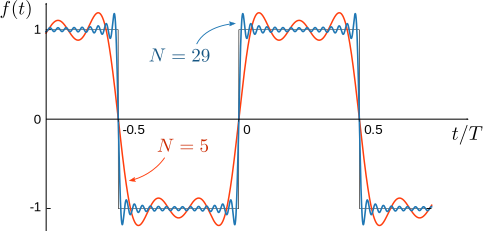
\includegraphics[width=0.55\textwidth]{square_fourier}
\end{center}
    

One amusing consequence of this result is that it can be used as a
series expansion for the mathematical constant $\pi$. If we set $x =
a/4$, then
\begin{equation}
  f(a/4) = 1 = \frac{4}{\pi}
  \left[\sin(\pi/2) + \frac{1}{3}\sin(3\pi/2) + \frac{1}{5}\sin(5\pi/2) + \cdots\right],
\end{equation}
and hence
\begin{equation}
  \pi = 4 \left(1 - \frac{1}{3} + \frac{1}{5} - \frac{1}{7} + \cdots\right).
\end{equation}

\section{Fourier transforms}\label{fourier-transforms}

The Fourier series discussed in the \hyperref[fourier-series]{previous
  section} applies to periodic functions, $f(x)$, defined over the
interval $-a/2 \le x < a/2$.  This concept can be generalized to
functions defined over the entire real line, $x \in \mathbb{R}$, by
carefully taking the limit $a \rightarrow \infty$.

Consider what happens when we apply the $a \rightarrow \infty$ limit
to the right-hand side of the
\hyperref[complex-fourier-series]{complex Fourier series formula from
  Section~\ref{complex-fourier-series}}:
\begin{equation}
  f(x) = \lim_{a\rightarrow \infty} \left( \sum_{n=-\infty}^\infty e^{i k_n x}\, f_n\right),
  \quad\mathrm{where}\;\; k_n = n\Delta k, \;\; \Delta k = \frac{2\pi n}{a}.
\end{equation}
As $a \rightarrow \infty$, the wave-number quantum $\Delta k$ goes to
zero. Hence, the set of values of $k_n$ turns into a continuum, and we
can replace the discrete sum with an integral over the values of
$k_n$. To do this, we multiply the summand by a factor of $(\Delta
k/2\pi) / (\Delta k/2\pi) = 1$:
\begin{equation}
  f(x) = \lim_{a\rightarrow \infty} \left[\;\,\sum_{n=-\infty}^\infty
    \frac{\Delta k}{2\pi} \, e^{i k_n x}\, \left(\frac{2\pi f_n}{\Delta k} \right)\;\,\right].
\end{equation}
If we now define
\begin{equation}
  F(k_n) \equiv \frac{2\pi}{\Delta k}\,f_n,
\end{equation}
then the sum becomes
\begin{equation}
  f(x) = \lim_{a\rightarrow \infty} \left( \sum_{n=-\infty}^\infty
  \frac{\Delta k}{2\pi} \, e^{i k_n x}\, F(k_n)\right).
\end{equation}
This limiting expression matches the basic definition of an integral:
\begin{equation}
  f(x) = \int_{-\infty}^{\infty} \frac{dk}{2\pi} \, e^{i k x}\, F(k).
\end{equation}
In case you're wondering, the factor of $2\pi$ is essentially
arbitrary, and is just a matter of how we chose to define $F(k_n)$.
Our choice corresponds to the standard definition of the Fourier
transform.

\subsection{The Fourier relations}
\label{fourier-relations}

The function $F(k)$ defined in the
\hyperref[fourier-transforms]{previous section} is called the
\textbf{Fourier transform} of $f(x)$. Just as we have expressed $f(x)$
in terms of $F(k)$, we can also express $F(k)$ in terms of $f(x)$. To
do this, we apply the $a \rightarrow \infty$ limit to the
\hyperref[complex-fourier-series]{inverse relation for the Fourier
  series (see Section~\ref{complex-fourier-series})}:
\begin{align}
  F(k_n) &= \lim_{a\rightarrow \infty} \frac{2 \pi}{\Delta k}\, f_n \\
  &= \lim_{a\rightarrow \infty} \frac{2 \pi}{2\pi/a}\, \left(\frac{1}{a}
  \int_{-a/2}^{a/2} dx\; e^{-i k_n x}\right) \\
  &= \int_{-\infty}^\infty dx\; e^{-i kx}\, f(x).
\end{align}
Hence, we arrive at a pair of equations called the \textbf{Fourier
  relations}:
\begin{align}
  \left\{\;\;\begin{aligned}F(k) &= \;\int_{-\infty}^\infty dx\; e^{-ikx}\, f(x) \\
  f(x) &= \int_{-\infty}^\infty \frac{dk}{2\pi}\; e^{ikx}\, F(k)\end{aligned}\;\;\right\}
\end{align}
The first equation is the Fourier transform, and the second equation
is called the \textbf{inverse Fourier transform}. These relations
state that if we have a function $f(x)$ defined over $x \in
\mathbb{R}$, then there is a unique counterpart function $F(k)$
defined over $k \in \mathbb{R}$, and vice versa. The Fourier transform
converts $f(x)$ to $F(k)$, and the inverse Fourier transform does the
reverse.

It is important to note the small differences between the two
formulas.  Firstly, there is a factor of $1/2\pi$ that ``tags along''
with $dk$, but not with $dx$; this is a matter of convention, tied to
our definition of $F(k)$, as mentioned before. Secondly, the integral
over $x$ contains a factor of $e^{-ikx}$ but the integral over $k$
contains a factor of $e^{ikx}$. One way to remember this is to think
of the integral over $k$, in the inverse Fourier transform equation,
as the continuum limit of a sum over complex waves, with $F(k)$
playing the role of the series coefficients; by convention, these
complex waves have the form $\exp(ikx)$.

In our definition of the Fourier transform, it is clear that the
Fourier series needs to remain convergent as we take the $a
\rightarrow \infty$ limit. Based on \hyperref[square-integrable]{our
  earlier discussion of square-integrable functions (Section
  \ref{square-integrable})}, this means we always deal with functions
such that
\begin{equation}
  \int_{-\infty}^{\infty} dx\; \big|\,f(x)\,\big|^2
\end{equation}
exists and is finite.

\subsection{A simple example}
\label{simple-example}

Consider the function
\begin{equation}
  f(x) = \left\{\begin{array}{cl}e^{-\eta x}, & x \ge 0 \\
  0, & x < 0,\end{array}\right. \qquad \eta \in \mathbb{R}^+.
\end{equation}
For $x < 0$, this is an exponentially-decaying function, and for $x <
0$ it is identically zero. The real parameter $\eta$ is called the
decay constant; for $\eta > 0$, the function $f(x)$ vanishes as $x
\rightarrow +\infty$ and can thus be shown to be square-integrable,
and larger values of $\eta$ correspond to faster exponential decay.

The Fourier transform can be found by directly calculating the Fourier
integral:
\begin{equation}
  F(k) \;=\; \;\int_{0}^\infty dx\; e^{-i kx}\, e^{-\kappa x} \;=\; \frac{-i}{k - i \eta}.
\end{equation}
It is useful to plot the squared magnitude of the Fourier transform,
$|F(k)|^2$, against $k$. This is called the \textbf{Fourier spectrum}
of $f(x)$. In this case,
\begin{equation}
  \big|\,F(k)\,\big|^2 = \frac{1}{k^2 + \eta^2}.
\end{equation}
This is plotted in the right-hand figure below:

\begin{figure}[h]
  \centering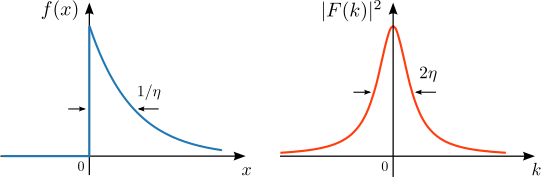
\includegraphics[width=0.6\textwidth]{fourier_example1}
\end{figure}

We call such a graph a \textbf{Lorentzian} curve.  It consists of a
peak centered at $k = 0$, whose height and width are dependent on the
decay constant $\eta$. For small $\eta$, i.e.~weakly-decaying $f(x)$,
the peak is high and narrow. For large $\eta$, i.e.~rapidly-decaying
$f(x)$, the peak is low and broad. This kind of relationship between
the decay rate and the Fourier spectrum peak width is very common.

    
We can quantify the width of the Lorentzian curve by defining the
\textbf{full-width at half-maximum} (FWHM), which is the width of the
curve at half the value of its maximum. In this case, the maximum of
the Lorentzian curve occurs at $k=0$ and has the value of $1/\eta^2$.
The half-maximum, $1/2\eta^2$, occurs when $\delta k = \pm \eta$.
Hence, the original function's decay constant, $\eta$, is directly
proportional to the FWHM of the Fourier spectrum, which is $2\eta$.

Note also that this relationship is dimensionally consistent. In
$f(x)$, the exponent $\eta x$ needs to be dimensionless, so the decay
constant has unit of $[1/x]$. This has the same units as the
wave-number variable $k$, which is the horizontal axis for the Fourier
spectrum.

To wrap up this example, let's evaluate the inverse Fourier transform:
\begin{equation}
  f(x) \; = \; -i\int_{-\infty}^\infty \frac{dk}{2\pi} \; \frac{e^{i kx}}{k-i\eta}.
\end{equation}
This can be done by contour integration (Chapter 8). The analytic
continuation of the integrand has one simple pole, at $k = i\eta$. For
$x < 0$, the numerator $\exp(ikx)$ blows up far from the origin in the
upper half of the complex plane, and vanishes far from the origin in
the lower half-plane; hence we close the contour in the lower
half-plane. This encloses no pole, so the integral is zero. For $x >
0$, the numerator vanishes far from the origin in the upper
half-plane, so we close the contour in the upper half-plane (i.e., the
contour is counter-clockwise). Hence,
\begin{equation}
  f(x) = \left(\frac{-i}{2\pi}\right) \, \left(2\pi i\right)
  \, \mathrm{Res}\left[ \frac{e^{ikx}}{k-i\eta}\right]_{k=i\eta} = e^{-\eta x} \qquad(x > 0)
\end{equation}
which is indeed the function that we started out with.

\subsection{Fourier transforms for time-domain functions}
\label{fourier_time}

Thus far, we have been dealing with functions of a spatial coordinate
$x$. Of course, these mathematical relations don't care about the
physical meaning of the variables, so the Fourier transform concept is
also applicable to functions of time $t$. However, there is a
vexatious difference in convention that needs to be observed: when
dealing with functions of the time coordinate $t$, it is customary to
use a different sign convention in the Fourier relations!

The Fourier relations for a function of time, $f(t)$, are:
\begin{align}
\left\{\;\,\begin{aligned}F(\omega) &= \;\int_{-\infty}^\infty dt\; e^{i\omega t}\, f(t) \\
f(t) &= \int_{-\infty}^\infty \frac{d\omega}{2\pi}\; e^{-i\omega t}\, F(\omega).\end{aligned}\;\,\right\}
\end{align}
These relations differ in one notable way from the Fourier relations
between $f(x)$ and $F(k)$ discussed in
\hyperref[fourier-relations]{Section~\ref{fourier-relations}}: the
signs of the $\pm i \omega t$ exponents are flipped.

There's a good reason for this difference in sign convention: it
arises from the need to describe propagating waves, which vary with
both space \emph{and} time. As we discussed in Chapter~5, a
propagating plane wave can be described by a wavefunction
\begin{equation}
  f(x,t) = A e^{i(kx - \omega t)},
\end{equation}
where $k$ is the wave-number and $\omega$ is the frequency. We write
the plane wave function this way so that positive $k$ indicates
forward propagation in space (i.e., in the $+x$ direction), and
positive $\omega$ indicates forward propagation in time (i.e., in the
$+t$ direction). This requires the $kx$ and $\omega t$ terms in the
exponent to have opposite signs, so that when $t$ increases by a
certain amount, a corresponding \emph{increase} in $x$ leaves the
total exponent unchanged.

Now, as we have seen, the inverse Fourier transform relation describes
how a wave-form is broken up into a superposition of elementary waves.
In the case of a wavefunction $f(x,t)$, the superposition is given in
terms of plane waves:
\begin{equation}
f(x,t) = \int_{-\infty}^\infty \frac{dk}{2\pi} \int_{-\infty}^\infty \frac{d\omega}{2\pi}\;\; e^{i(kx-\omega t)}\, F(k,\omega).
\end{equation}
To be consistent with this, we need to treat space and time variables
with oppositely-signed exponents:
\begin{align}
  f(x) &= \int_{-\infty}^\infty \frac{dk}{2\pi}\; e^{ikx}\, F(k) \\
  f(t) &= \int_{-\infty}^\infty \frac{d\omega}{2\pi}\; e^{-i\omega t}\, F(\omega).
\end{align}
The other set of Fourier relations follow from this choice.

\subsection{Basic properties of the Fourier transform}
\label{fourier-properties}

The Fourier transform has several properties that are useful to
remember. These can all be directly proven using the definition of the
Fourier transform.  The proofs are left as exercises.

\begin{enumerate}[(i)]
\item 
The Fourier transform is linear: if we have two functions $f(x)$ and
$g(x)$, whose Fourier transforms are $F(k)$ and $G(k)$ respectively,
then for any constants $a, b \in \mathbb{C}$,
\begin{equation}
a f(x) + b g(x) \;\;\;  \overset{\mathrm{FT}}{\longrightarrow} \;\;\; a F(k) + b G(k).
\end{equation}

\item
Performing a coordinate translation on a function causes its Fourier
transform to be multiplied by a ``phase factor'':
\begin{equation}
f(x+b) \;\;\;  \overset{\mathrm{FT}}{\longrightarrow} \;\;\; e^{ikb} \, F(k).
\end{equation}
As a consequence, translations leave the Fourier spectrum $|F(k)|^2$
unchanged.

\item
If the Fourier transform of $f(x)$ is $F(k)$, then
\begin{equation}
f^*(x) \quad  \overset{\mathrm{FT}}{\longrightarrow} \;\; F^*(-k).
\end{equation}
As a consequence, the Fourier transform of a real function must
satisfy the symmetry relation $F(k) = F^*(-k)$, meaning that the
Fourier spectrum is symmetric about the origin in k-space:
$\big|\,F(k)\,\big|^2 = \big|\,F(-k)\,\big|^2.$

\item
When you take the derivative of a function, that is equivalent to
multiplying its Fourier transform by a factor of $ik$:
\begin{equation}
\frac{d}{dx} f(x) \,\;\;  \overset{\mathrm{FT}}{\longrightarrow} \;\;\; ik F(k).
\end{equation}
For functions of time, because of the
\hyperref[fourier_time]{difference in sign convention
  (Section~\ref{fourier_time})}, there is an extra minus sign:
\begin{equation}
  \frac{d}{dt} f(t) \;\;\;\;  \overset{\mathrm{FT}}{\longrightarrow} \;\;\; -i\omega F(\omega).
\end{equation}
\end{enumerate}

\subsection{Fourier transforms of differential equations}
\label{fourier-transforms-of-differential-equations}

The Fourier transform can be a very useful tool for solving
differential equations. As an example, consider a damped harmonic
oscillator that is subjected to an additional driving force $f(t)$.
This force has an arbitrary time dependence, and is not necessarily
harmonic. The equation of motion is
\begin{equation}
  \frac{d^2 x}{dt^2} + 2\gamma \frac{dx}{dt} + \omega_0^2 x(t) = \frac{f(t)}{m}.
\end{equation}
To solve for $x(t)$, we first take the Fourier transform of both sides
of the above equation. The result is:
\begin{equation}
  - \omega^2 X(\omega) - 2 i\gamma \omega X(\omega) + \omega_0^2 X(\omega) = \frac{F(\omega)}{m},
\end{equation}
where $X(\omega)$ and $F(\omega)$ are the Fourier transforms of $x(t)$
and $f(t)$ respectively. To obtain the left-hand side of this
equation, we made use of the \hyperref[fourier-properties]{properties
  of the Fourier transform described in
  Section~\ref{fourier-properties}}, specifically linearity (i) and
Fourier transformations of derivatives (iv). Note also that we have
used the sign convention for time-domain functions
\hyperref[fourier_time]{discussed in Section~\ref{fourier_time}}.

The Fourier transform has turned our ordinary differential equation
into an algebraic equation. This equation can be easily solved:
\begin{equation}
  X(\omega) = \frac{F(\omega)/m}{- \omega^2 - 2 i\gamma \omega + \omega_0^2}
\end{equation}
Knowing $X(\omega)$, we can use the inverse Fourier transform to
obtain $x(t)$.

To summarize, the solution procedure for the driven harmonic
oscillator equation consists of (i) using the Fourier transform on
$f(t)$ to obtain $F(\omega)$, (ii) using the above equation to find
$X(\omega)$ algebraically, and (iii) performing an inverse Fourier
transform to obtain $x(t)$. This will be the basis for the Green's
function method, a method for systematically solving differential
equations that will be discussed later.

\section{Common Fourier transforms}
\label{common-fourier-transforms}

To accumulate more intuition about Fourier transforms, we will now study
the Fourier transforms of a few interesting functions. We will simply
state the results, leaving the actual calculations of the Fourier
transforms as exercises.

\subsection{Damped waves}\label{damped-waves}

\hyperref[simple-example]{In Section~\ref{simple-example}}, we saw
that an exponentially decay function with decay constant $\eta \in
\mathbb{R}^+$ has the following Fourier transform:
\begin{equation}
  f(x) = \left\{\begin{array}{cl}e^{-\eta x}, & x \ge 0 \\ 0, & x < 0,\end{array}\right. \;\;  \overset{\mathrm{FT}}{\longrightarrow} \;\; F(k) = \frac{-i}{k-i\eta}.
\end{equation}
Observe that $F(k)$ is given by a simple algebraic formula. If we
``extend'' the domain of $k$ to complex values, $F(k)$ corresponds to
an analytic function with a simple pole in the upper half of the
complex plane, at $k = i\eta$.

Next, consider a decaying wave with wave-number $q \in \mathbb{R}$ and
decay constant $\eta \in \mathbb{R}^+$. The Fourier transform is a
function with a simple pole at $q + i \eta$:
\begin{equation}
f(x) = \left\{\begin{array}{cl}e^{i (q + i\eta) x}, & x \ge 0 \\ 0, & x < 0.\end{array}\right. \;\;  \overset{\mathrm{FT}}{\longrightarrow} \;\; F(k) = \frac{-i}{k-(q + i\eta)}.
\end{equation}
Hence, the Fourier spectrum is 
\begin{equation}
  |F(k)|^2 = \frac{1}{(k-q)^2 + \eta^2}.
\end{equation}
This is a Lorentzian peaked at $k = q$ and having width $2\eta$, as
shown below:

\begin{figure}[h]
  \centering\includegraphics[width=0.65\textwidth]{fourier_example2}
\end{figure}

On the other hand, consider a wave that grows exponentially with $x$
for $x < 0$, and is zero for $x > 0$. The Fourier transform is a
function with a simple pole in the lower half-plane:
\begin{equation}
  f(x) = \left\{\begin{array}{cl}0, & x \ge 0 \\
  e^{i (q - i\eta) x}, & x < 0.\end{array}\right. \;\;
  \overset{\mathrm{FT}}{\longrightarrow} \;\; F(k) = \frac{i}{k-(q - i\eta)}.
\end{equation}
The Fourier spectrum is, likewise, a Lorentzian centered at $k = q$.

\begin{figure}[h]
  \centering\includegraphics[width=0.65\textwidth]{fourier_example3}
\end{figure}

From these examples, we see that oscillations and amplification/decay
in $f(x)$ are related to the existence of poles in the algebraic
expression for $F(k)$. The real part of the pole position gives the
wave-number of the oscillation, and the distance from the pole to the
real axis gives the amplification or decay constant. A decaying signal
produces a pole in the upper half-plane, while a signal that is
increasing exponentially with $x$ produces a pole in the lower
half-plane. In both cases, if we plot the Fourier spectrum of
$|F(k)|^2$ versus real $k$, the result is a Lorentzian curve centered
at $k = q$, with width $2\eta$.

\subsection{Gaussian wave-packets}\label{gaussian-wave-packets}

It is also interesting to look at the Fourier transform of a function
that decays faster than an exponential. In particular, let's consider
a function with a decay ``envelope'' given by a Gaussian function:
\begin{equation}
  f(x) = e^{iq x} \, e^{-\gamma x^2}, \;\;\;\mathrm{where}\;
  q \in \mathbb{C},\; \gamma \in \mathbb{R}.
\end{equation}
Such a function is called a \textbf{Gaussian wave-packet}. The width
of the Gaussian envelope can be characterized by the Gaussian
function's ``standard deviation'', which is where the curve reaches
$e^{-1/2}$ times its peak value.  In this case, the standard deviation
is $\Delta x = 1/\sqrt{2\gamma}$.

It can be shown that $f(x)$ has the following Fourier transform:
\begin{equation}
  F(k) = \sqrt{\frac{\pi}{\gamma}} \, e^{-\frac{(k-q)^2}{4\gamma}}.
\end{equation}
To derive this result, we perform the Fourier integral as follows:
\begin{align}
  F(k) &= \int_{-\infty}^\infty dx \, e^{-ikx}\, f(x) \\
  &= \int_{-\infty}^\infty dx \, \exp\left\{-i(k-q)x -\gamma x^2\right\}.
\end{align}
In the integrand, the expression inside the exponential is quadratic
in $x$. We complete the square:
\begin{align}
  F(k) &= \int_{-\infty}^\infty dx \,
  \exp\left\{-\gamma\left(x + \frac{i(k-q)}{2\gamma}\right)^2
  + \gamma\left(\frac{i(k-q)}{2\gamma}\right)^2\right\} \\
  &= \exp\left\{ - \frac{(k-q)^2}{4\gamma}\right\}\; \int_{-\infty}^\infty dx
  \, \exp\left\{-\gamma\left(x + \frac{i(k-q)}{2\gamma}\right)^2\right\}.
\end{align}
The remaining integral is simply the Gaussian integral (see Chapter
2), with a constant shift in $x$ which can be eliminated by a change
of variables. This yields the result stated above.

The Fourier spectrum, $|F(k)|^2$, is a Gaussian function with standard
deviation
\begin{equation}
  \Delta k = \frac{1}{\sqrt{2(1/2\gamma)}} = \sqrt{\gamma}.  
\end{equation}

\begin{figure}[h]
  \centering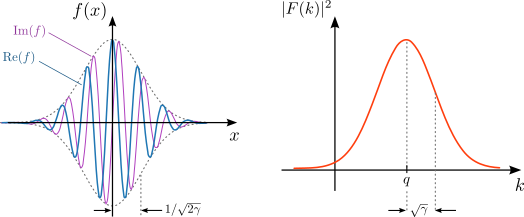
\includegraphics[width=0.65\textwidth]{fourier_example4}
\end{figure}

Thus, we again see that the Fourier spectrum is peaked at a value of
$k$ corresponding to the wave-number of the underlying sinusoidal wave
in $f(x)$. Moreover, a stronger (weaker) decay in $f(x)$ leads to a
broader (narrower) Fourier spectrum.

\section{The delta function}\label{delta-function}

What happens when we feed the Fourier relations into one another?
Plugging the Fourier transform into the inverse Fourier transform, we
get
\begin{align}
  f(x) &= \int_{-\infty}^\infty \frac{dk}{2\pi} \, e^{ikx} F(k) \\
  &= \int_{-\infty}^\infty \frac{dk}{2\pi} \, e^{ikx} \int_{-\infty}^\infty dx' e^{-ikx'} f(x')\\
  &= \int_{-\infty}^\infty dx' \int_{-\infty}^\infty \frac{dk}{2\pi} \, e^{ikx} e^{-ikx'} f(x')\\
  &= \int_{-\infty}^\infty  dx' \; \delta(x-x')\, f(x').
\end{align}
In the last step, we have introduced
\begin{equation}
  \delta(x-x') = \int_{-\infty}^\infty \frac{dk}{2\pi} \, e^{ik(x-x')},
\end{equation}
which is called the \textbf{delta function}. According to the above
equations, the delta function acts as a kind of filter: when we
multiply it by any function $f(x')$ and integrate over $x'$, the
result is the value of that function at a particular point $x$.

But here's a problem: the above integral definition of the delta
function is non-convergent; in particular, the integrand does not vanish
at $\pm \infty$. We can get around this by thinking of the delta
function as a limiting case of a convergent integral. Specifically,
let's take
\begin{equation}
  \delta(x-x') = \lim_{\gamma \rightarrow 0} \, \int_{-\infty}^\infty \frac{dk}{2\pi} \, e^{ik(x-x')} \, e^{-\gamma k^2}.
\end{equation}
For $\gamma \rightarrow 0$, the ``regulator'' $\exp(-\gamma k^2)$
which we have inserted into the integrand goes to one, so that the
integrand goes back to what we had before; on the other hand, for
$\gamma > 0$ the regulator ensures that the integrand vanishes at the
end-points so that the integral is well-defined. But the expression on
the right is the \hyperref[gaussian-wave-packets]{Fourier transform
  for a Gaussian wave-packet (see
  Section~\ref{gaussian-wave-packets})}. Using that result, we get
\begin{equation}
  \delta(x-x') = \lim_{\gamma \rightarrow 0} \; \frac{1}{\sqrt{4\pi\gamma}} \,
  e^{-\frac{(x-x')^2}{4\gamma}}.
\end{equation}
This is a Gaussian function, with standard deviation $\sqrt{2\gamma}$
and area $1$. Hence, the delta function can be regarded as the limit
of a Gaussian function as its width goes to zero while keeping the
area under the curve fixed at unity (which means the height of the
peak goes to infinity).

The most important feature of the delta function is it acts as a
``filter''. Whenever it shows up in an integral, it picks out the
value of the rest of the integrand evaluated where the delta function
is centered:
\begin{equation}
  \int_{-\infty}^\infty  dx \; \delta(x-x_0)\, f(x) = f(x_0).
\end{equation}
Intuitively, we can understand this behavior from the above definition
of the delta function as the zero-width limit of a Gaussian. When we
multiply a function $f(x)$ with a narrow Gaussian centered at $x_0$,
the product will approach zero almost everywhere, because the Gaussian
goes to zero. The product is non-zero only in the vicinity of $x =
x_0$, where the Gaussian peaks. And because the area under the delta
function is unity, integrating that product over all $x$ simply gives
the value of the other function at the point $x_0$.

\section{Multi-dimensional Fourier transforms}
\label{multi-dimensional-fourier-transforms}

When studying problems such as wave propagation, we will often have to
deal with Fourier transforms acting on several variables
simultaneously.  This is conceptually straightforward. For a function
$f(x_1, x_2, \dots, x_d)$ which depends on $d$ independent spatial
coordinates $x_1, x_2, \dots x_d$, we can simply perform a Fourier
transform on each coordinate individually:
\begin{equation}
  F(k_1, k_2, \dots, k_d) = \int_{-\infty}^\infty dx_1\; e^{-ik_1x_1}\;
  \int_{-\infty}^\infty dx_2\; e^{-ik_2x_2}\,\cdots\, \int_{-\infty}^\infty dx_d\;
  e^{-ik_d x_d}\, f(x_1,x_2, \dots,x_N)
\end{equation}
Note that each coordinate gets Fourier-transformed into its own
independent $k$ variable, so that the result is still a function of
$d$ independent variables.

We can compactly express such a ``multi-dimensional Fourier
transform'' via vector notation. Let $\vec{x} = [x_1, x_2, \dots,
  x_d]$ be a $d$-dimensional coordinate vector. The
Fourier-transformed coordinates can be written as $\vec{k} = [k_1,
  k_2, \dots, k_d]$, and the Fourier transform is
\begin{equation}
  F(\vec{k}) = \int_{-\infty}^\infty dx_1\, \int_{-\infty}^\infty dx_2 \cdots
  \int_{-\infty}^\infty dx_d\; e^{-i\,\vec{k}\,\cdot\,\vec{x}}\, f(\vec{x}),
\end{equation}
where $\vec{k}\cdot\vec{x} \equiv k_1 x_1 + k_2 x_2 + \cdots + k_d
x_d$ is the usual dot product of two vectors.

The inverse Fourier transform is
\begin{equation}
  f(\vec{x}) = \int_{-\infty}^\infty \frac{dk_1}{2\pi}\, \int_{-\infty}^\infty
  \frac{dk_2}{2\pi} \cdots \int_{-\infty}^\infty \frac{dk_d}{2\pi}\;
  e^{i\,\vec{k}\,\cdot\,\vec{x}}\, F(\vec{k}).
\end{equation}
A multi-dimensional \hyperref[delta-function]{delta function} can be
defined as the Fourier transform of a plane wave:
\begin{equation}
  \delta^d(\vec{x}-\vec{x}') = \int_{-\infty}^\infty \frac{dk_1}{2\pi}
  \int_{-\infty}^\infty \frac{dk_2}{2\pi} \cdots \int_{-\infty}^\infty
  \frac{dk_d}{2\pi} \, e^{i\vec{k} \cdot \left(\vec{x}-\vec{x}'\right)}.
\end{equation}
Note that $\delta^d$ has the dimensions of $[x]^{-d}$. The
multi-dimensional delta function has a ``filtering'' property similar
to the one-dimensional delta function.  For any $f(x_1,\dots,x_d)$,
\begin{equation}
  \int_{-\infty}^\infty dx_1 \cdots \int_{-\infty}^\infty dx_d \; \delta^d(\vec{x}-\vec{x}')
  \, f(\vec{x}) = f(\vec{x}').
\end{equation}

Finally, if we have a mix of spatial and temporal coordinates, then
the \hyperref[fourier_time]{usual sign conventions (see
  Section~\ref{fourier_time})} apply to each individual
coordinate. For example, if $f(x,t)$ is a function of one spatial
coordinate and one temporal coordinate, the Fourier relations are
\begin{align}
  F(k, \omega) &= \int_{-\infty}^\infty dx\; \int_{-\infty}^\infty dt\;
  e^{-i(kx-\omega t)}\; f(x,t) \\
  f(x, t) &= \int_{-\infty}^\infty \frac{dk}{2\pi}\; \int_{-\infty}^\infty
  \frac{d\omega}{2\pi}\; e^{i(kx-\omega t)}\; F(k,\omega).
\end{align}

\section{Exercises}

\begin{enumerate}
\item 
Find the relationship between the coefficients $\{\alpha_n, \beta_m\}$
in the sine/cosine Fourier series and the coefficients $f_n$ in the
complex exponential Fourier
series:
\begin{align}
  f(t) &= \sum_{n=1}^\infty \alpha_n \sin\left(\frac{2\pi n x}{a}\right)
  + \sum_{m=0}^\infty \beta_m \cos\left(\frac{2 \pi m x}{a}\right) \\
  &= \sum_{n=-\infty}^\infty f_n \exp\left(\frac{2\pi i n x}{a}\right).
\end{align}

\item
Find the Fourier series expansion of the triangular
wave
\begin{equation}
f(x) = \left\{\begin{array}{rr}-c x, &-a/2 \le x < 0, \\ c x, & 0 \le x < a/2\end{array}\right.
\end{equation}
where $c$ is some real constant. Using the result, derive a series
expansion for $\pi^2$.

\item
Prove the properties of the Fourier transform listed in
\hyperref[fourier-properties]{Section~\ref{fourier-properties}}.

\item
Find the Fourier transform of $f(x) = \sin(\kappa x)/x.$

\item
Prove that if $f(x)$ is a real function, then its Fourier transform
satisfies $F(k) = F(-k)^*$.
\end{enumerate}

\end{document}
